\chapter{Résultats obtenus}
%---------------------------------------------------------------------------------------------------------------
\section{Films et mots}

En développant petit à petit nos extractions, nos créations de matrices, nous avons pu analyser certaines choses. Notamment, nous trouvons intéressant de voir combien de mots uniques se retrouvent dans les descrptifs de films en fonction du nombre de films que nous tenons en compte. La figure \ref{wordsmoviefunction} montre un courbe qui arbore une tendence logarithmique. Cela est le cas avec nos mesures, mais il serait intéressant de voir avec encore plus de films pour savoir si cette tendance se vérifie.

\begin{figure}[h]
  \centering
    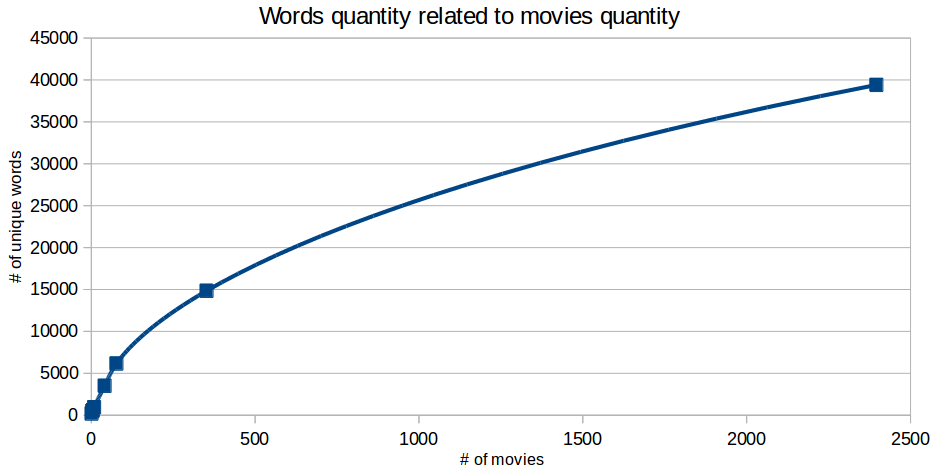
\includegraphics[width=0.9\linewidth]{img/wordsmoviefunction.png}
  \caption{Nombre de mots uniques en fonction du nombre de films}
  \label{wordsmoviefunction}
\end{figure}


%---------------------------------------------------------------------------------------------------------------
\section{Optimisations}

Comme dit plus haut, la première optimisation a été de supprimer les mots qui ne se trouvent que dans un seul film. Pour le fichier contenant les 2396 films, nous avions 57'987 mots avant l'optimisation et nous nous retrouvons avec 39'404 mots après. Dans l'opération, 18'583 mots ont été supprimés. Nous pouvons le voir dans les histogrammes de la figure \ref{histooccurrence}, tous les mots qui avaient une seule occurrence ont disparus.

\begin{figure}[h!]
    \centering
    \begin{tabular}{cc}
      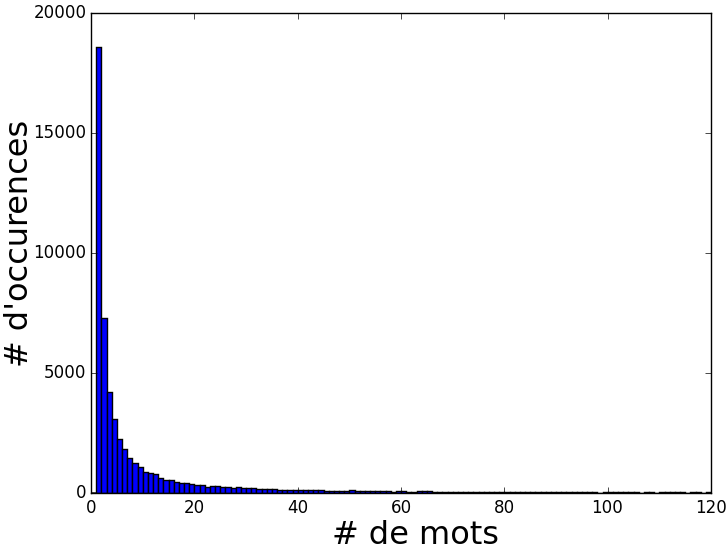
\includegraphics[width=.5\linewidth]{img/data3-3393-120.png} &
      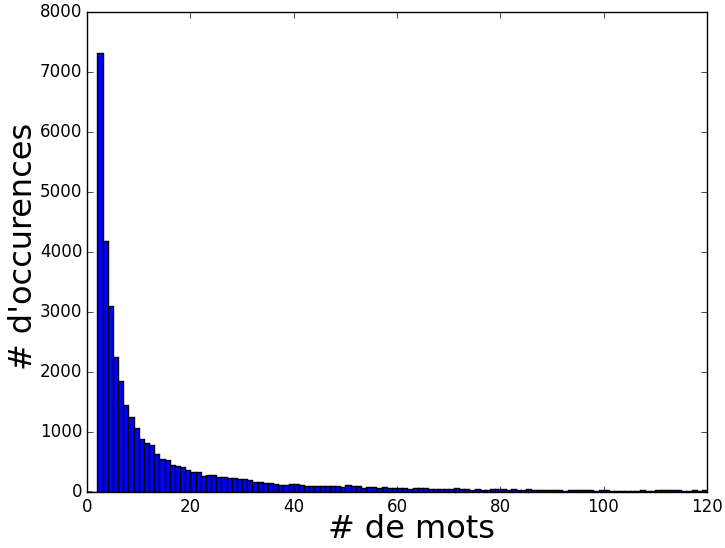
\includegraphics[width=.5\linewidth]{img/data4-3393-120.png} \\
      (a) & (b)\\
    \end{tabular}
    \caption{Histogramme du nombre de mots qui ont les mêmes occurrences (a) normal (b) après suppression des mots uniques
    \label{histooccurrence}}
\end{figure}

Les histogrammes montrent les occurrences jusqu'à 120. Après vérification, nous avons vu que le mot avec le plus d'occurrences en avait 25'802. Cela est énorme et n'a pas beaucopu de valeur. Il y a deux possibilités : soit il s'agit d'un \textit{stop word}, soit c'est un terme qui est vraiment utilisé souvent et dans beaucoup de films. Dans les deux cas, il serait bien de supprimer ces mots. Nous pourrions filtrer à partir d'un certain nombre d'occurrence pour rendre les résultats plus pertinents. Il faut faire attention à ne pas filtrer les termes important par contre.


%---------------------------------------------------------------------------------------------------------------
\section{Liste des films similaires}

Les résultats de la liste des films similaires à ``Witness for the Prosecution'' sont les suivants : \\

\begin{lstlisting}[language=python]
  Witness for the Prosecution:Crime,Drama,Mystery,Thriller :

  0 Witness for the Prosecution:Crime,Drama,Mystery,Thriller

  1 A Few Good Men:Crime,Drama,Mystery,Thriller

  2 Touch of Evil:Crime,Film-Noir,Thriller

  3 Chaplin:Biography,Drama

  4 Breaking the Waves:Drama,Romance

  5 Before the Devil Knows Youre Dead:Crime,Drama,Thriller

  6 Mercury Rising:Action,Crime,Drama,Thriller

  7 The Graduate:Comedy,Drama,Romance

  8 Scary Movie:Comedy

  9 Femme Fatale:Crime,Thriller
\end{lstlisting}

On peut voir que la catégorie du film sélectionné est "Crime,Drama,Mystery,Thriller" et on voit que les films détectés comme similaires ont des catégories en commun. On peut en déduire que l'algorithme semble reconnaître assez bien les films similaires.

%---------------------------------------------------------------------------------------------------------------
\section{Clustering hiérarchique}

Les résultats du clustering hiérarchique sont montrés à la figure \ref{hierarchical} ci-dessous.

\begin{figure}[h]
  \centering
    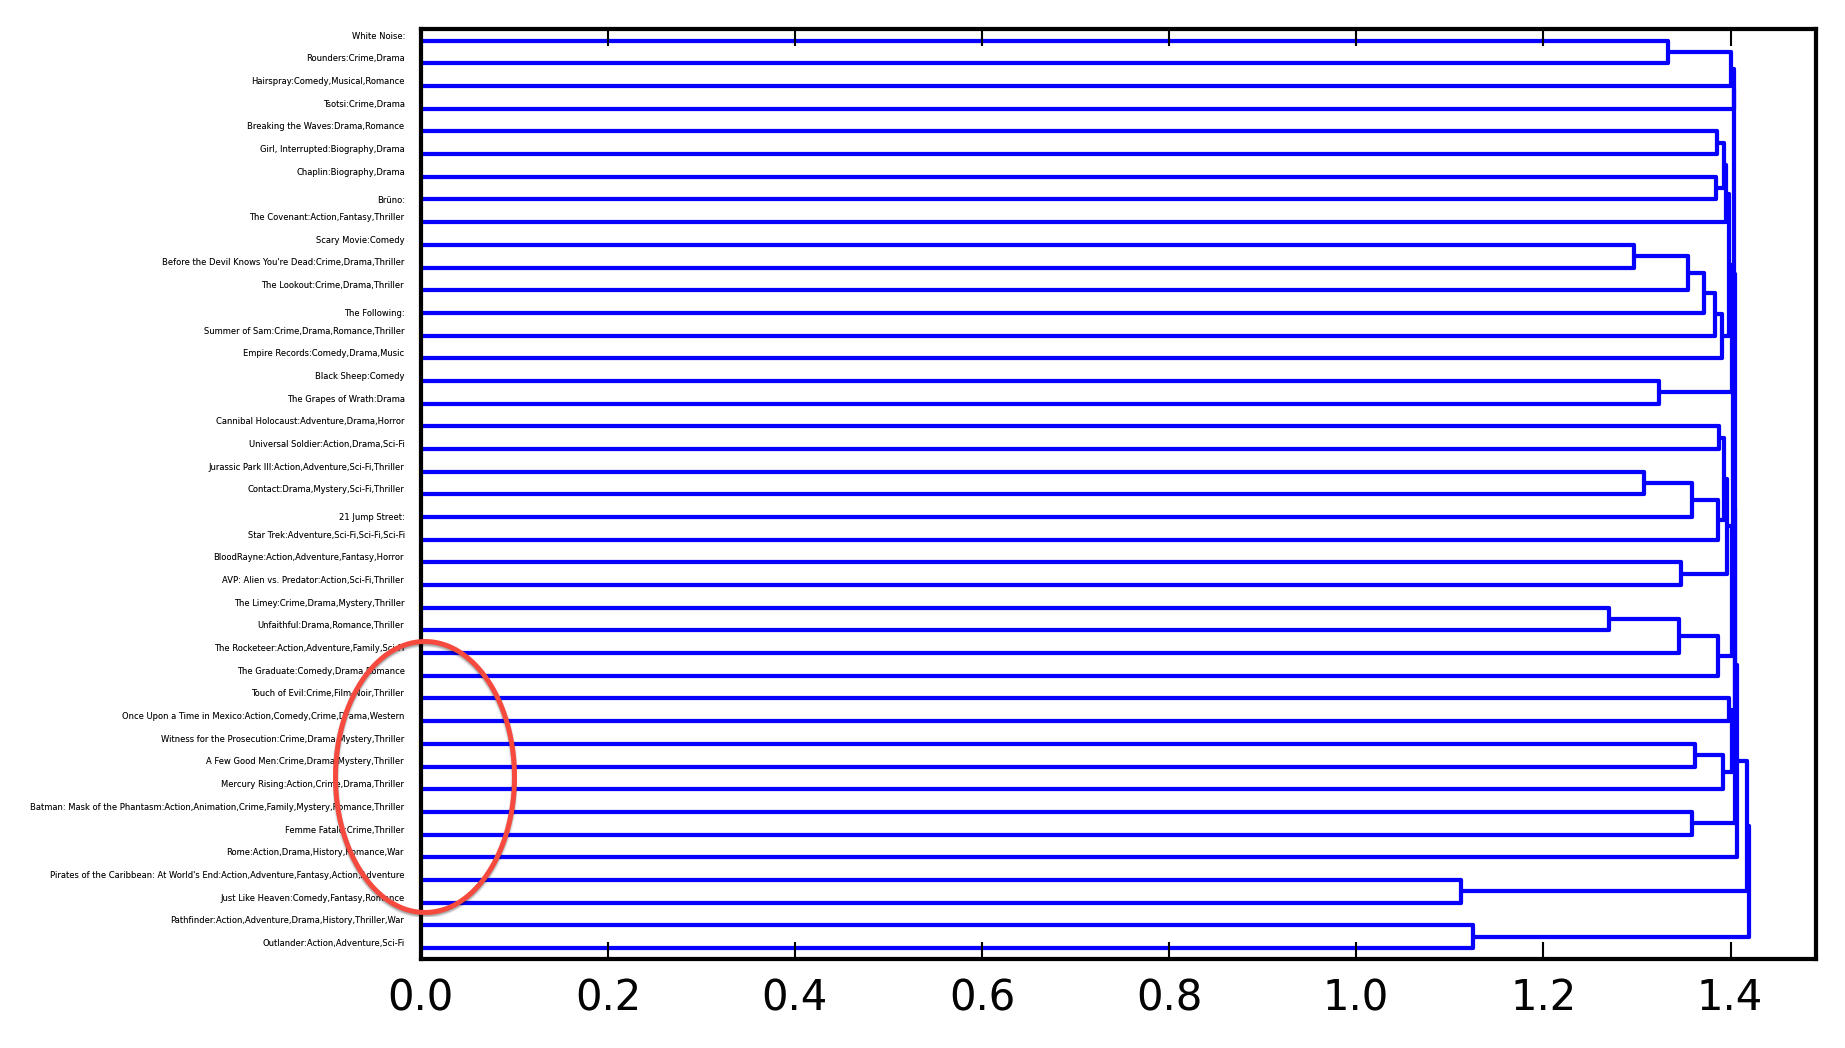
\includegraphics[width=1\linewidth]{img/clustering50_tf_idf.png}
  \caption{Dendogram du clustering hiérarchique}
  \label{hierarchical}
\end{figure}

En faisant un zoom sur l'image (figure \ref{zoom}) on peut voir quel film a été groupé et on peut voir sa catégorie. Dans l'image ci-dessous on peut voir comme les films de la même catégorie ont été groupés ensemble.

\begin{figure}[h]
  \centering
    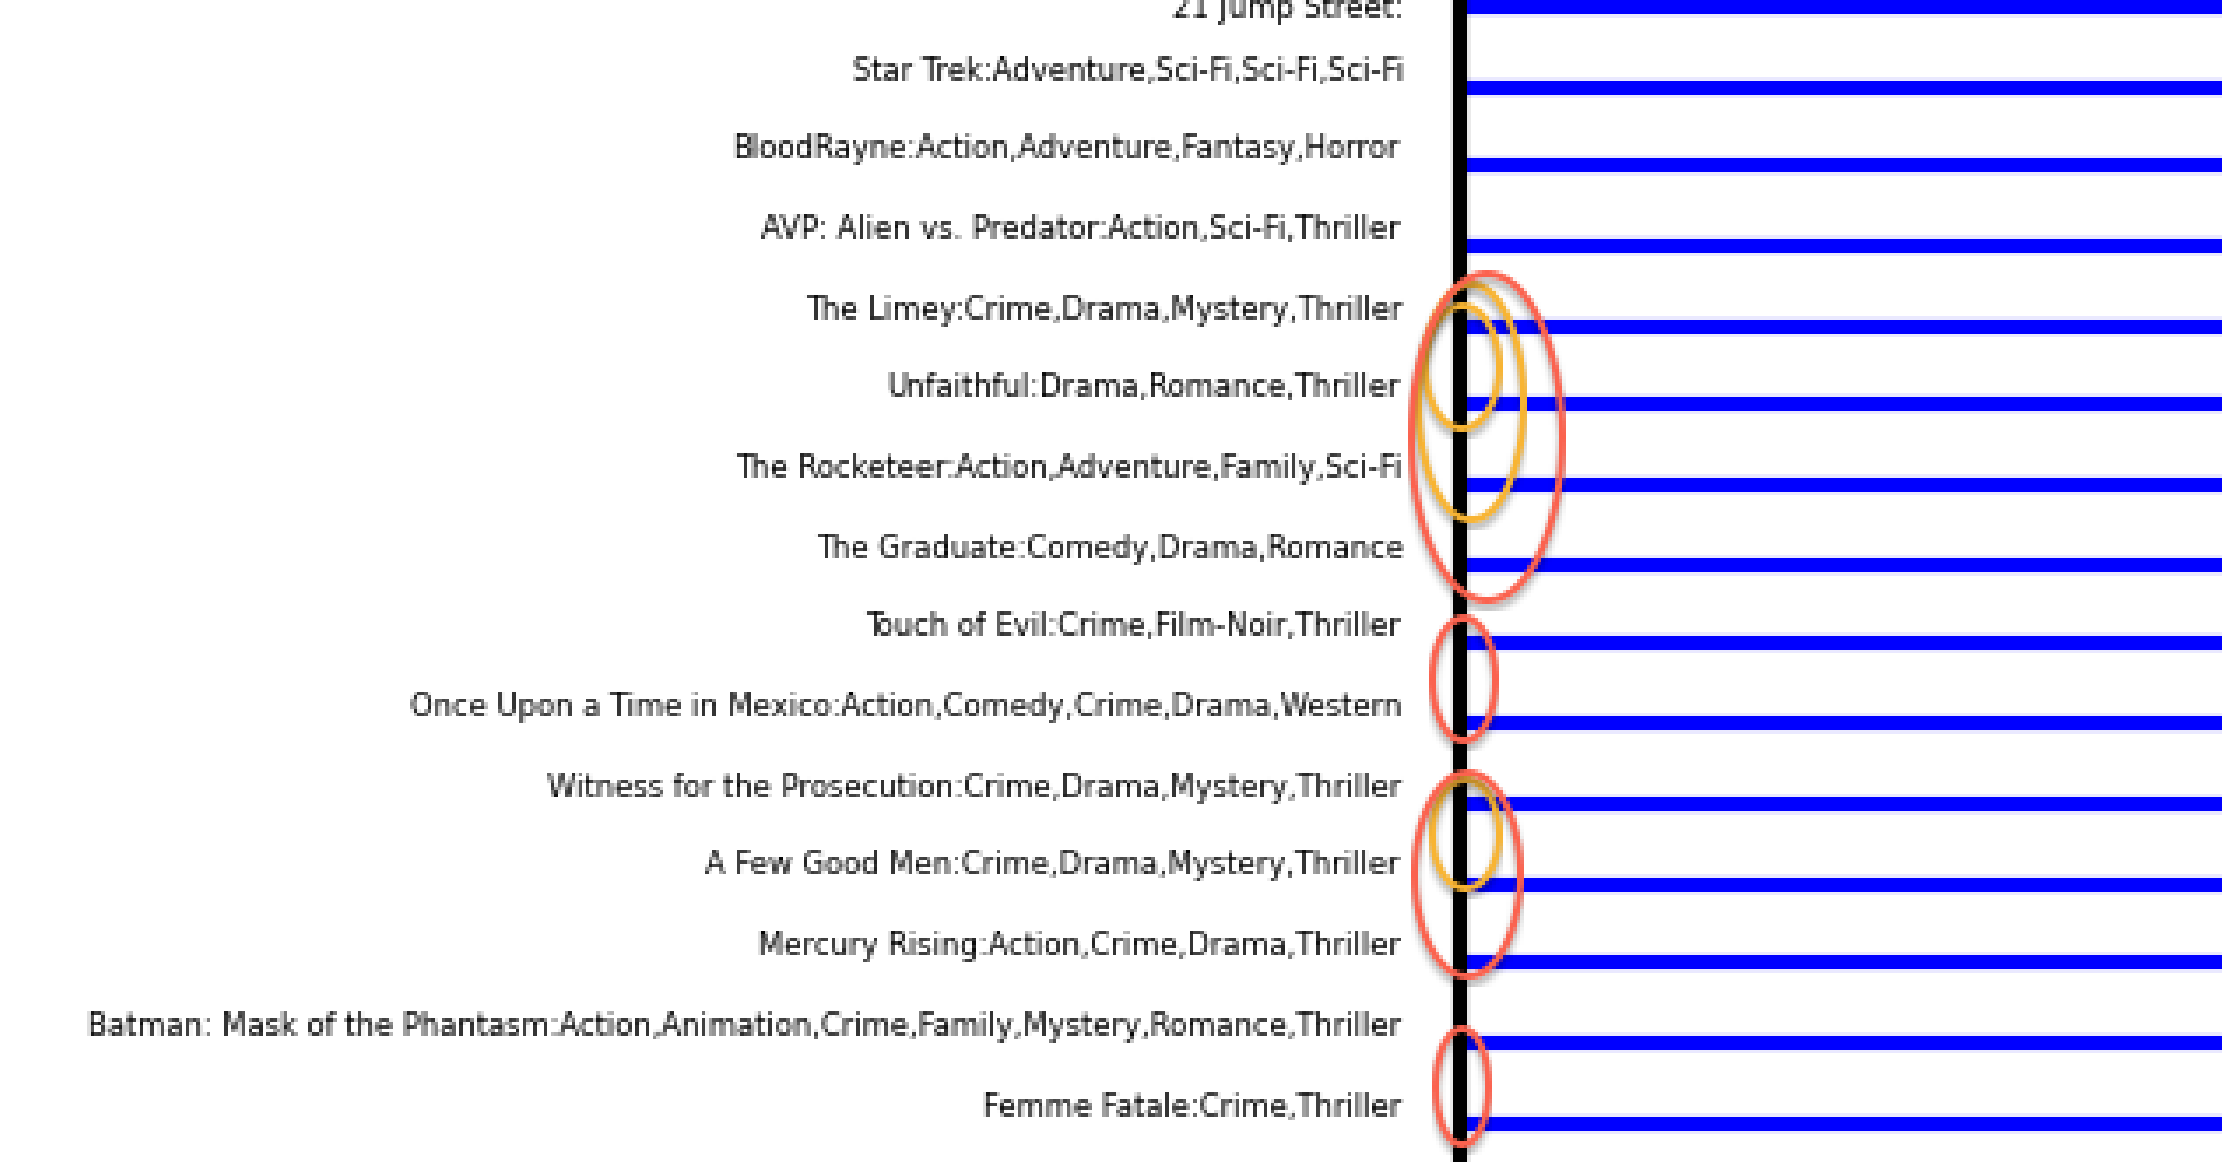
\includegraphics[width=1\linewidth]{img/zoom.png}
  \caption{Dendogram du clustering hiérarchique, zoom}
  \label{zoom}
\end{figure}
\newpage
%Pour les films sans catégorie on peut cette fois les imaginer en regardant le groupement que l'algorithme a fait. Pour le film "Bruno" (figure \ref{bruno}) on peut en ne déduire que c'est similaire à "Chaplin" et qui aura une catégorie similaire a "Biography, Drama" ou peut-être il's ont simplement la description du film similaire. Peut-être aussi de ce deux films sont définissent une nouvelle catégorie. En regardant sur IMDB et en recherchant sur Wikipedia on peut voire qu’effectivement le film Bruno est un comédie drôle qui parle du personnage Bruno. On peut donc confirmer qui appartiens aussi à la catégorie "Biographie".
%Pour les films sans catégorie on peut cette fois les imaginer en regardant le groupement que l'algorithme a fait. Pour le film "White noise" (figure \ref{whitenoise}) on peut en ne déduire que c'est similaire à "Rounders" et qui aura une catégorie similaire a "Crime, Drama" ou peut-être il's ont simplement la description du film similaire. Peut-être aussi de ce deux films sont définissent une nouvelle catégorie. En regardant sur IMDB et en recherchant sur Wikipedia on peut voire effectivement le film "White noise" est dans les catégories "Drama, Mystery" c'est qui c'est donc vraisemblable avec notre résultats.
Dans les clusters créés il y a aussi "Scary Movie" qui est groupé avec "Before the Devil Knows You're Dead" (figure \ref{scarymovie}) qui ont des catégories complètement différentes. Mais, si on regarde le synopsis des deux, on peut voir qu’il y a beaucoup de mots qui sont en commun entre les deux films. Plus précisément, les deux films ont les mots "Bobby, Ray, kill" avec une fréquence très haute dans les deux synopsis. Ce qui explique leur similarité. De plus, le film "Scary Movie" est une parodie de film d'horreur, c'est donc la raison pour laquelle on trouve beaucoup de mot en commun dans les deux synopsis.
 
\begin{figure}[h]
  \centering
    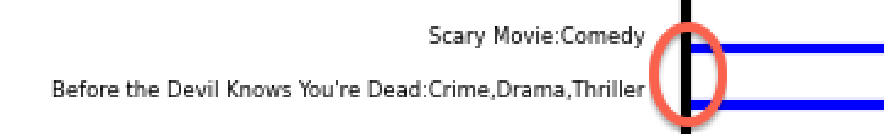
\includegraphics[width=0.5\linewidth]{img/scarymovie.png}
  \caption{``Scary Movie'' et ``Before the Devil Knows You're Dead''}
  \label{scarymovie}
\end{figure}



%---------------------------------------------------------------------------------------------------------------
\section{Map de Kohonen}

Après avoir vu que l'algorithme est capable de reconnaître les films avec une description similaire on peut utiliser un algorithme plus avancé pour avoir en sortie une carte des films. Ces films sont organisés sur la carte en fonction des ressemblances qu'ils ont avec les autres. Les couleurs de la carte représentent la distance entre chaque film. Une couleur rouge indique que la distance est grande et une couleur bleue indique le contraire. La figure \ref{map1} montre un exemple d'une carte générée avec 100 films.

\begin{figure}[h]
  \centering
  \includegraphics[width=1\linewidth]{img/map-cluster.png}
  \caption{Map de Kohonen avec 100 films}
  \label{map1}
\end{figure}

On peut voir avec les couleurs de l'image qu'il a des zones délimitées par de rouge, comme l'angle en bas à gauche. Il y a aussi des zones délimitées par du vert ou jaune. La division en rouge indique que la division est beaucoup plus forte que celle en jaune. Si on agrandit l'image on pourra voir le groupe des films similaires que la map de Kohonen a créé.
Dans l'image agrandie de la figure \ref{map1zoom2} on peut voir qu'il y a des groupes dans l'angle en bas à gauche. On peut voir que l'algorithme a placé dans la même région (cercle rouge) les films "Bloody Rayne", "Alien vs Predator" et "Cannibal Holocaust". Ces films ont des catégories en commun. On peut en déduire que la description de ces deux films est effectivement similaire.

Dans l'ellipse orange on peut voir un autre groupe formé sur la map de Kohonen qui regroupe les films d'action, d'aventure et dramatiques.

\begin{figure}[h]
	\centering
	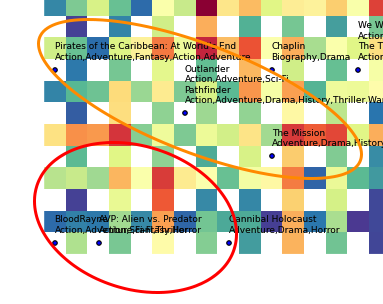
\includegraphics[width=0.5\linewidth]{img/map1zoom2.png}
	\caption{Map de Kohonen avec le zoom de l'angle en bas à gauche}
	\label{map1zoom2}
\end{figure}

\newpage
Dans l'autre coté de l'image (figure \ref{map1zoom3}) on peut voir un autre groupe des films. On voit que cette fois on regroupe les films avec les catégories "Crime , Drama, Comedy, Biography". Même si les catégories sont légèrement différentes on doit penser que la reconnaissance est faite sur la description du film et pas sur d'autre paramètre de plus haut niveau.

\begin{figure}[h]
\centering
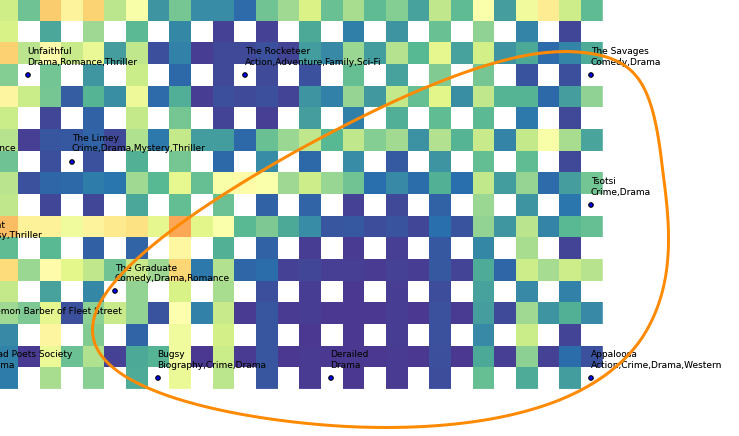
\includegraphics[width=0.6\linewidth]{img/map1zoom3.png}
\caption{Map de Kohonen avec le zoom de l'angle en bas à droite}
\label{map1zoom3}
\end{figure}


%---------------------------------------------------------------------------------------------------------------
% Code integration example
%\begin{lstlisting}[language=bash]
%  sudo apt-get update
%  sudo apt-get install drupal7
%\end{lstlisting}

% Image integration example
%\begin{figure}[h]
%  \centering
%    \includegraphics[width=1\linewidth]{img/drupalFirstPage.png}
%  \caption{Page d'accueil du site créé avec Drupal sur une instance EC2}
%  \label{drupalfirstpage}
%\end{figure}

% Image side-by-side
%\begin{figure}[h!]
%    \centering
%    \begin{tabular}{cccc}
%      \includegraphics[width=.14\linewidth]{randomTree_n5.png} &
%      \includegraphics[width=.22\linewidth]{randomTree_n10.png} &
%      \includegraphics[width=.22\linewidth]{randomTree_n15.png} \\
%      (a) & (b) & (c)\\
%    \end{tabular}
%    \caption{Arbres aléatoires où (a) n=5 (b) n=10 (c) n=15
%    \label{randomTrees}}
%\end{figure}